Trabaje para $t\ge0$ con la transformada unilateral de Laplace y entradas causales. Use $H(t-a)=0$ para $t<a$ y $H(t-a)=1$ para $t\ge a$; los valores aislados en saltos no alteran la transformada. Sea
\[f(t)=\begin{cases}2\sin t,&0\le t<\pi,\\0,&t\ge\pi.\end{cases}\]
La gráfica de $g$ es una versión de este semiseno con las escalas de tiempo y amplitud indicadas; fuera del arco es cero.
\begin{center}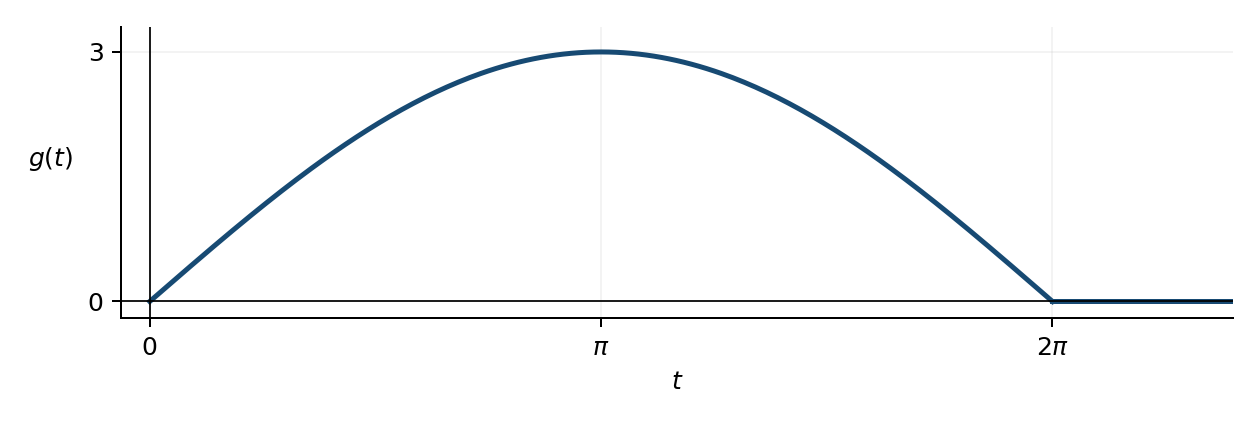
\includegraphics[width=.9\linewidth]{assets/M2-E0227-input.png}\end{center}

\begin{enumerate}[label=(\alph*),ref=\alph*,leftmargin=*]
\item Calcule la transformada de $f$.
\item Utilizando el apartado anterior, calcule la transformada de $g$.
\item Resuelva $y''-4y=f(t)$, $y(0)=0$, $y'(0)=1$.
\end{enumerate}
